\section{Biopython \& Scipy} \label{sec:MAFFT}

The colored cluster trees were created by \textbf{ETE3} with a newick file, generated using a feature request, proposed for the scipy package as described in the issue\footnote{\url{https://github.com/scipy/scipy/issues/8274} (last accessed 06/02/21)} (\autoref{fig:Tree_Pipeline} \textsf{\textbf{J}}).

Clusters centroid vectors were selected by calculating euclidean distance between all the vectors of a cluster to each other. The vector with the minimum mean of overall distance was declared as centroid (\autoref{fig:Tree_Pipeline} \textsf{\textbf{K}}). 

The materials described in the following were only used for the analyses in the \autoref{sec:Clustering_Anomalies} to \autoref{sec:Dimension_Reduction} and are, therefore, not included in the novel \gls{IAV} clustering tool (\autoref{fig:Alignment_Pipeline} and \autoref{fig:Precalc_Pipeline}).

All precalculated trees were also created by using the same mentioned vector distance calculation using cosine distance calculation on the L1-norm normalized k-mer frequency vectors instead (\autoref{fig:Precalc_Pipeline} \textsf{\textbf{F}}). The calculated distances were used for \gls{UPGMA} tree building with tree construction functions of the biopython package. DistanceMatrix function was used with standard settings and DistanceTreeConstructor with \texttt{method='upgma'} (\autoref{fig:Alignment_Pipeline} \textsf{\textbf{O}} and \textsf{\textbf{P}}) \autocite{gower_minimum_1969}. The vectors were also clustered by \gls{HDBSCAN} using the calculated distances with \texttt{metric='precalculated'}. Other settings were used as described in \autoref{sec:HDBSCAN} without hybrid clustering.

\begin{figure}[!hbt]
    \centering
    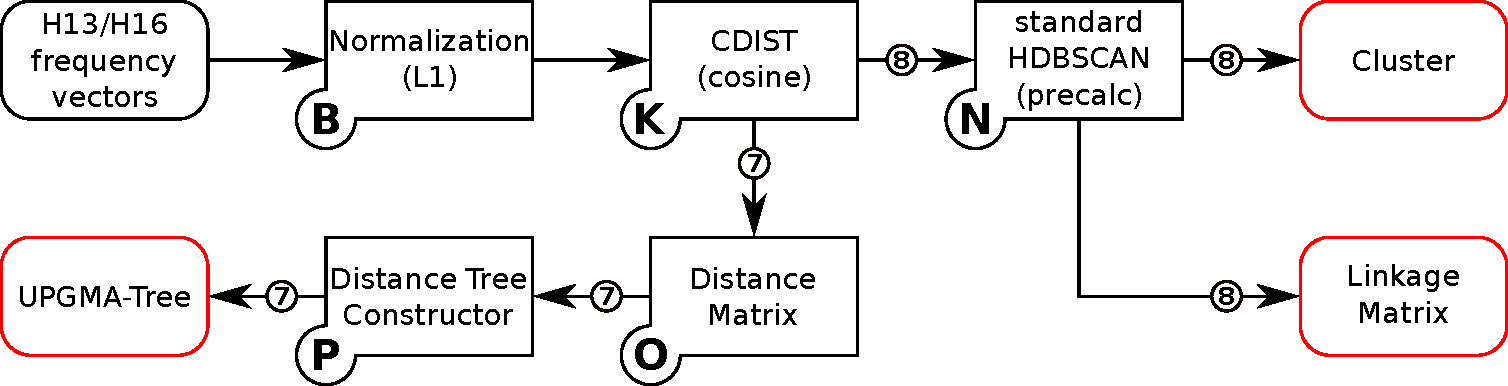
\includegraphics[width=\textwidth]{Graphics/Precalculated.pdf}
    \caption[Precalculation Pipeline]{\textbf{Precalculation Pipeline.} For the precalculated trees the L1-normalized k-mer vectors were compared by cosine distance prior to clustering by \gls{HDBSCAN} and on the other hand processing with \textbf{biopython (Bio)} package \gls{UPGMA} calculation and visualization by \textbf{ETE3}.}
    \label{fig:Precalc_Pipeline}
\end{figure}

MAFFT was used for \glspl{MSA} and guide tree creation with \texttt{treeout=True} on the centroid sequences and on a small FASTA subset (\autoref{fig:Alignment_Pipeline} \textsf{\textbf{L}}) \autocite{katoh_mafft_2013}. The \gls{MSA} of the FASTA subset was converted to evolutionary distances with DistanceCalculator of the biopython package using standard settings and clustered by \gls{HDBSCAN} similar to the cosine distances (\autoref{fig:Alignment_Pipeline} \textsf{\textbf{M}} and \textsf{\textbf{N}}). PairwiseAligner also from the biopython packages was used for the pairwise alignments in \autoref{sec:Serotype_Classification}.

\begin{figure}[!hbt]
    \centering
    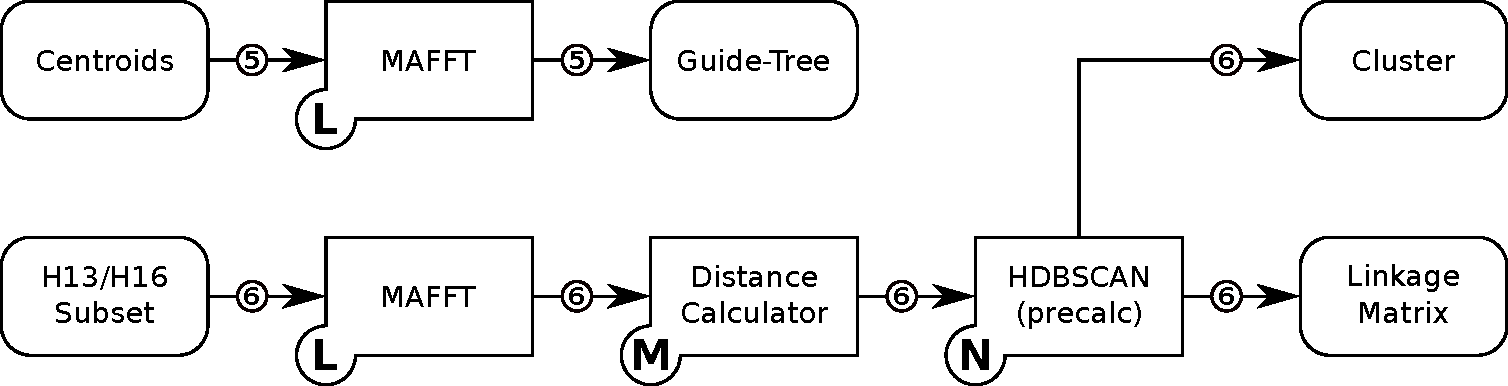
\includegraphics[width=\textwidth]{Graphics/Alignment.pdf}
    \caption[Alignment Pipeline]{\textbf{Alignment Pipeline.} The analysis steps involving \glspl{MSA} are performed as pictured. The sequences related to the centroids were aligned using MAFFT resulting in the output as guide-tree visualized by \textbf{ETE3}. The small subset for comparison was also aligned by MAFFT prior to evolutionary distance calculation and clustering by \gls{HDBSCAN}.}
    \label{fig:Alignment_Pipeline}
\end{figure}






For the pairwise alignments in \autoref{sec:Serotype_Classification} from the \textbf{biopython (Bio)} package version 1.78, the \textbf{Align.PairwiseAligner} function was used with standard settings \autocite{cock_biopython_2009}. 

Important parameters used in this project, including settings varying from the default, are listed below. All available settings with explanation are listed in the \href{https://biopython.org/docs/1.75/api/Bio.Align.html}{API}.

The Biopython implementation of MAFFT version 7.475 from the \textbf{biopython (Bio)} package version 1.78 was used to build the guide trees in \autoref{sec:Clustering_Anomalies} according to \autoref{fig:Alignment_Pipeline} pathway \textsf{\textbf{5}} with the genomic sequences of the centroids $C$ \autocite{katoh_mafft_2013, cock_biopython_2009} (\autoref{fig:Alignment_Pipeline}. The settings were the default settings proposed in the \href{https://mafft.cbrc.jp/alignment/software/}{manual}, with changes in the thread number and the output format. For faster execution \colorbox{backcolour}{thread=6} and for export of the guide tree \colorbox{backcolour}{treeout=True} setting was used \autocite{katoh_mafft_2013, cock_biopython_2009}. The guide-tree was colored with \textbf{ETE3} (\autoref{fig:Alignment_Pipeline} \textsf{\textbf{K}}) \autocite{huerta-cepas_ete_2016}.

Important parameters used in this project, including settings varying from the default, are listed below. All available settings with explanation are listed in the \href{https://mafft.cbrc.jp/alignment/software/}{manual}.

% \begin{leftbar}
%     %\textbf{mafft}
%     \textbf{Bio.Align.Applications.MafftCommandline}
%     \begin{nstabbing}
%         \qquad\qquad\qquad\qquad\qquad\quad\=\kill
    
%         treeout \> [export guide tree used for alignment (default: off)]\\
        
%         thread \> [number of used threads (default: 1)]\\
        
%         input \> [input FASTA file]
        
%         %-{}-{}6merpair \> (default: on)\\
%         %\> input\\
%         %> \> output
%     \end{nstabbing}
% \end{leftbar}

In \autoref{sec:Comparison_Clustering} five different cluster trees are compared to each other. The trees are based on clustering with \gls{HDBSCAN}, without hybrid clustering ($\varepsilon=0$) \autocite{malzer_hybrid_2020, mcinnes_hdbscan_2017}. For each clustering a different matrix was used as input. The trees of \gls{UMAP} and \gls{PCA} (\autoref{fig:Simple_Clustertree_PCA} and \autoref{fig:Simple_Clustertree_UMAP}) were created according to \autoref{fig:Vectorization_Pipeline} and \autoref{fig:Clustering_Pipeline} and as described in \autoref{sec:Frequency} to \autoref{sec:HDBSCAN} with a smaller FASTA subset $S$ containing only segment 4 sequences with subtypes H13 and H16 and a resulting smaller L2-norm normalized \gls{PCA} matrix $\mathbf{X}_{\text{L2}}$ and smaller \gls{UMAP} matrix $\mathbf{Y}_{\text{L2}}$. Clustering for the trees of \gls{UMAP} and \gls{PCA} was performed similar to \autoref{sec:HDBSCAN} but without $\varepsilon$ with the small matrix variants of $\mathbf{X}_{\text{L2}}$ and $\mathbf{Y}_{\text{L2}}$ (\autoref{eq:hdb_prime_x} and \autoref{eq:hdb_prime_y}). 

% \begin{empheq}{alignat = -1}
%     &N_{\text{UMAP}} &&= \text{HDBSCAN} (\mathbf{X}_{\text{L2}}, 2, 1, 0)\label{eq:hdb_prime_x}\\
%     &N_{\text{PCA}} &&= \text{HDBSCAN} (\mathbf{Y}_{\text{L2}}, 2, 1, 0)\label{eq:hdb_prime_y}
% \end{empheq}

The two trees based the clustering with precalculation (\autoref{fig:Simple_Clustertree_Cosine} and \autoref{fig:Simple_Clustertree_Euclid}) were created by distance calculation on the L1-norm normalized matrix $\mathbf{X}_{\text{L1}}$ of the smaller $S$. For the calculation of the distance the \textbf{scipy} package version 1.6.0 was used with the \textbf{spatial.distance.cdist} function (\autoref{fig:Precalc_Pipeline} \textsf{\textbf{N}}) \autocite{scipy_10_contributors_scipy_2020}. For calculation of the cosine distance \colorbox{backcolour}{metric='cosine'} and for euclidean distance \colorbox{backcolour}{metric='euclidean'} setting was used (\autoref{eq:c_calc_matrix} to \autoref{eq:e_calc_matrix}). The resulting distance matrices $\mathbf{C}$ and $\mathbf{E}$ were clustered with \gls{HDBSCAN} and \colorbox{backcolour}{metric='precalculated'} setting (\autoref{fig:Precalc_Pipeline} \textsf{\textbf{F}} and \autoref{eq:hdb_prime_e} to \autoref{eq:hdb_prime_c}) \autocite{mcinnes_hdbscan_2017}.

% \begin{empheq}{alignat = -1}
%     &c_{i,j} &&= d_{\text{cos}}(\mathbf{x}_i, \mathbf{x}_j), \ i = 1, \ldots o, \ j = 1, \ldots o\label{eq:c_calc_1}\\
%     &&&= 1 - \frac{\mathbf{x}_i^\top\mathbf{x}_j}{\Vert\mathbf{x}_i\Vert \cdot \Vert\mathbf{x}_j\Vert}\label{eq:c_calc_2}
% \end{empheq}

% \begin{empheq}{alignat = -1}
%     &\mathbf{C} &&= \text{CDIST}_{\text{cosine}}(\mathbf{X}_{\text{L1}}, \mathbf{X}_{\text{L1}}) \label{eq:c_calc_matrix}\\
%     &\mathbf{E} &&= \text{CDIST}_{\text{euclidean}}(\mathbf{X}_{\text{L1}}, \mathbf{X}_{\text{L1}}) \label{eq:e_calc_matrix}
% \end{empheq}

% \begin{empheq}{alignat = -1}
%     &N_{\text{eucl}} &&= \text{HDBSCAN} (\mathbf{E}, 2, 1, 0)\label{eq:hdb_prime_e}\\
%     &N_{\text{cos}} &&= \text{HDBSCAN} (\mathbf{C}, 2, 1, 0)\label{eq:hdb_prime_c}
% \end{empheq}

% Important parameters used in this project, including settings varying from the default, are listed below. All available settings with explanation are listed in the \href{https://docs.scipy.org/doc/scipy/reference/generated/scipy.spatial.distance.cdist.html}{API}.

% \begin{leftbar}
%     \textbf{scipy.spatial.distance.cdist}
%     \begin{nstabbing}
%         \qquad\qquad\qquad\qquad\qquad\quad\=\kill
    
%         metric \> [Distance metric for calculation (default: 'euclidean')]

%     \end{nstabbing}
% \end{leftbar}

The \textbf{spatial.distance.cdist} function is also used for a fast pairwise alignment using the mentioned \textbf{Align.PairwiseAligner} above. Therefore, a small python definition containing the \textbf{Align.PairwiseAligner} function was inserted as metric setting into \textbf{spatial.distance.cdist}. 

The last of the five trees is based on MAFFT with the \textbf{biopython} package. The alignment was done on the subset $S$. On the alignment the distance matrix was calculated by the \textbf{Phylo.TreeConstruction.DistanceCalculator} function from the \textbf{biopython (Bio)} package. The standard settings for nucleotide sequences was used for the calculation \colorbox{backcolour}{model='identity'} \autocite{cock_biopython_2009}.

% \begin{empheq}{alignat = -1}
%     &\mathbf{G} &&= \text{DistanceCalculator}_{\text{identity}}(\text{MAFFT}(S_{\text{Sub}}))
% \end{empheq}

% \begin{empheq}{alignat = -1}
%     &N_{\text{msa}} &&= \text{HDBSCAN} (\mathbf{G}, 2, 1, 0)\label{eq:hdb_prime_g}
% \end{empheq}

% Important parameters used in this project, including settings varying from the default, are listed below. All available settings with explanation are listed in the \href{https://biopython.org/docs/latest/api/Bio.Phylo.TreeConstruction.html}{API}.

% \begin{leftbar}
%     \textbf{Bio.Phylo.TreeConstruction.DistanceCalculator}
%     \begin{nstabbing}
%         \qquad\qquad\qquad\qquad\qquad\quad\=\kill
    
%         model \> [model for distance calculation (default: 'identity')]

%     \end{nstabbing}
% \end{leftbar}

The \textbf{Phylo.TreeConstruction.DistanceMatrix} and \textbf{DistanceTreeConstructor} function, also from the \textbf{biopython} package, was used for calculation of precalculated UPGMA trees in \autoref{sec:K_mer_Representation}. Instead of the default neighbor joining setting, the bottom-up hierarchical clustering method \colorbox{backcolour}{method='upgma'} was used (\autoref{fig:Alignment_Pipeline} \textsf{\textbf{O}} and \textsf{\textbf{P}}) \autocite{gower_minimum_1969, cock_biopython_2009}. The matrices calculated in \autoref{eq:c_calc_matrix} and \autoref{eq:e_calc_matrix} were used as input for the calculation of the UPGMA-trees \autocite{sokal_statistical_1958}.

% Important parameters used in this project, including settings varying from the default, are listed below. All available settings with explanation are listed in the same \href{https://biopython.org/docs/latest/api/Bio.Phylo.TreeConstruction.html}{API} of \textbf{Bio.Phylo.TreeConstruction}.

% \begin{leftbar}
%     \textbf{Bio.Phylo.TreeConstruction.DistanceMatrix}
%     \begin{nstabbing}
%         \qquad\qquad\qquad\qquad\qquad\quad\=\kill
    
%         names \> [name of columns and rows]\\
        
%         matrix \> [input matrix]
%     \end{nstabbing}
% \end{leftbar}

% \begin{leftbar}
%     \textbf{Bio.Phylo.TreeConstruction.DistanceTreeConstructor}
%     \begin{nstabbing}
%         \qquad\qquad\qquad\qquad\qquad\quad\=\kill
    
%         method \> [construction method for the distance tree (default: 'nj')]
        
%     \end{nstabbing}
% \end{leftbar}